% Copyright 2002-2024 The University of Maryland Baltimore County (UMBC) and Richard J. Zak.
% 1000 Hilltop Circle, Baltimore, Maryland, 21250, USA
% https://www.csee.umbc.edu/
% richard.j.zak@gmail.com

\documentclass[letter,11pt]{article}
\usepackage[breaklinks]{hyperref}
\hypersetup{
    bookmarks=true,         % show bookmarks bar?
    unicode=false,          % non-Latin characters in Acrobat’s bookmarks
    pdftoolbar=true,        % show Acrobat’s toolbar?
    pdfmenubar=true,        % show Acrobat’s menu?
    pdffitwindow=false,     % window fit to page when opened
    pdfstartview={XYZ null null 1.00},    % disable zoom
    pdftitle={Linux @ UMBC},    % title
    pdfauthor={Richard Zak},     % author
    pdfsubject={Linux @ UMBC},   % subject of the document
    pdfkeywords={Computer Science, Programming, Linux, UMBC, CSEE}, % list of keywords
    pdfnewwindow=true,      % links in new PDF window
    colorlinks=false,       % false: boxed links; true: colored links
    linkcolor=red,          % color of internal links (change box color with linkbordercolor)
    citecolor=green,        % color of links to bibliography
    filecolor=magenta,      % color of file links
    urlcolor=cyan           % color of external links
}
\usepackage{graphicx}
\usepackage{placeins}
\usepackage{fancyhdr}
\usepackage{multicol}
\usepackage{xcolor}
\usepackage{tikz}
\pagestyle{fancy}
\usepackage[letterpaper, margin=1in]{geometry}
\geometry{letterpaper}
\usepackage{parskip} % Disable initial indent
\usepackage{color,soul} % Highligher
\usepackage[normalem]{ulem} % Strikethrough with \sout{}

\usepackage[utf8]{inputenc}
\fancyhf{}
\renewcommand{\headrulewidth}{0pt} % Remove default underline from header package
\rhead{Connecting to and Using UMBC's Linux Servers\begin{picture}(0,0) \put(85,-6){
\includegraphics[width=1.1cm]{Images/Tux.png}} \end{picture}}
%\rhead{}
\lhead{\begin{picture}(0,0) \put(0,-10){
\includegraphics[width=1.1cm]{Images/UMBC-vertical}} \end{picture}}
\cfoot{\thepage}
\rfoot{}
\lfoot{Linux @ UMBC}
\AtEndDocument{\vfill \footnotesize{Last updated 15 September 2021} \hfill \LaTeX}

\begin{document}

\tableofcontents

\section{Connecting}
\paragraph{Before you begin} There are many examples of commands which are to be typed into a command prompt or entered into a dialog box. Use common sense, and think before you enter commands. Don't blindly copy and paste commands expecting that something useful will result.

\subsection{Windows Users}
\FloatBarrier
\subsubsection{Putty}
\paragraph{}Putty is a Windows program which provides access to the command line interface on a UNIX system, which includes Linux. It's not the only program which can be used for this, but it's the easiest to use and most convenient.

\begin{enumerate}
    \item Start by downloading Putty from \url{https://www.chiark.greenend.org.uk/~sgtatham/putty/latest.html}. The Installer option adds the option to have a shortcut on the desktop. However, the \texttt{putty.exe} link under ``Alternative binary files'' provides the program itself, which you may place where you'd like.
    \item When you launch Putty, enter \texttt{gl.umbc.edu} in the ``Host Name'' field and click ``Open'', as shown in \autoref{fig:puttyconnection}.
    \item For the first time you connect, you'll see a box asking about caching the host key. Don't worry about this, click ``Yes'', as shown in \autoref{fig:puttyserverkey}.
    \item A black window will appear asking for your user name, then you'll see some text from UMBC, followed by a password prompt. Type your password, and it will not be shown. \autoref{fig:puttyconnected} shows what you'll see once connected.
\end{enumerate}

\begin{figure}
\centering
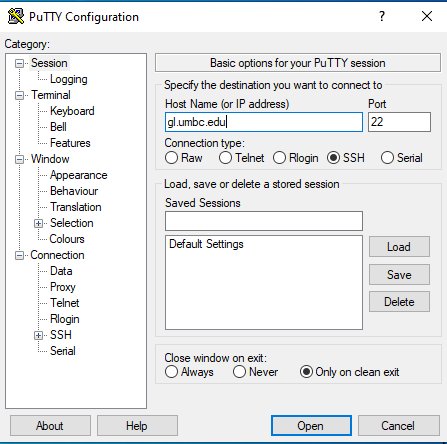
\includegraphics[scale=0.6]{Images/putty_connect_1.png}
\caption{The Putty connection dialog box.}
\label{fig:puttyconnection}
\end{figure}

\begin{figure}
\centering
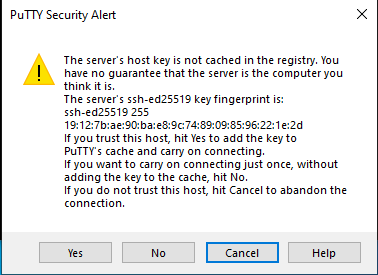
\includegraphics[scale=0.7]{Images/putty_connect_2_first_time.png}
\caption{Putty asking about the server SSH key.}
\label{fig:puttyserverkey}
\end{figure}

\begin{figure}
\centering
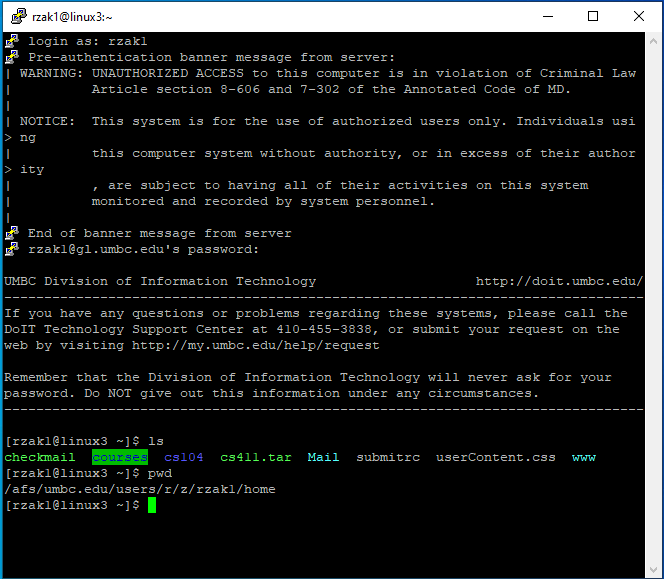
\includegraphics[scale=0.7]{Images/putty_connected.png}
\caption{Putty is connected to the Linux server.}
\label{fig:puttyconnected}
\end{figure}

\FloatBarrier
\subsubsection{WinSCP}
\paragraph{}Putty allows you to enter commands on the Linux command line interface, and WinSCP allows you to transfer files to and from the Linux environment using the familiar drag-and-drop interface.

\begin{enumerate}
    \item Start by downloading WinSCP from \url{https://winscp.net/eng/download.php}, which provides the installer. If you want to have a portable version which you can place anywhere, visit \url{https://winscp.net/eng/downloads.php}.
    \item Launch WinSCP and enter \texttt{gl.umbc.edu} in the ``Host name'' field, your user name \& password in the appropriate fields. Click ``Login''. An example is shown in \autoref{fig:winscpconnect}.
    \item Just as with Putty, the first time you connect, you'll be asked to accept the server's SSH key. Click ``Yes'', as shown in \autoref{fig:winscpconnectfirsttime}.
    \item Once connected, you'll see a two-pane window showing your local computer on the left, and the files \& directories (folders) on the right, as shown in \autoref{fig:winscpconnected}.
\end{enumerate}

\begin{figure}
\centering
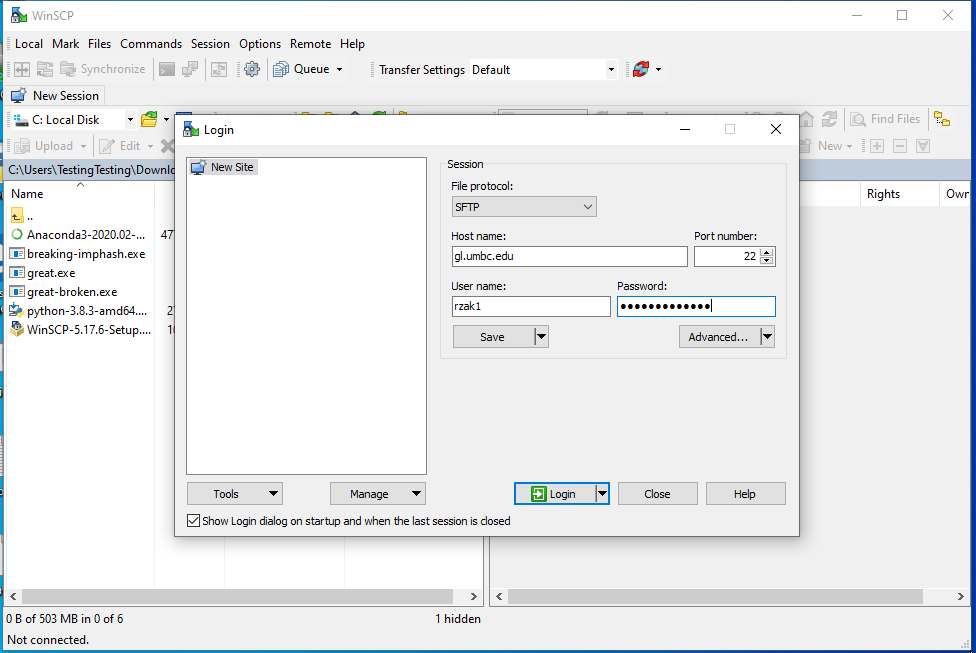
\includegraphics[scale=0.6]{Images/winscp_gl_connect.png}
\caption{WinSCP connection dialog box.}
\label{fig:winscpconnect}
\end{figure}

\begin{figure}
\centering
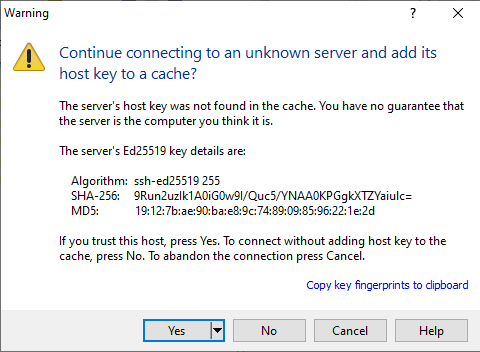
\includegraphics[scale=0.7]{Images/winscp_connect_first_time.png}
\caption{WinSCP asking about the server SSH key.}
\label{fig:winscpconnectfirsttime}
\end{figure}

\begin{figure}
\centering
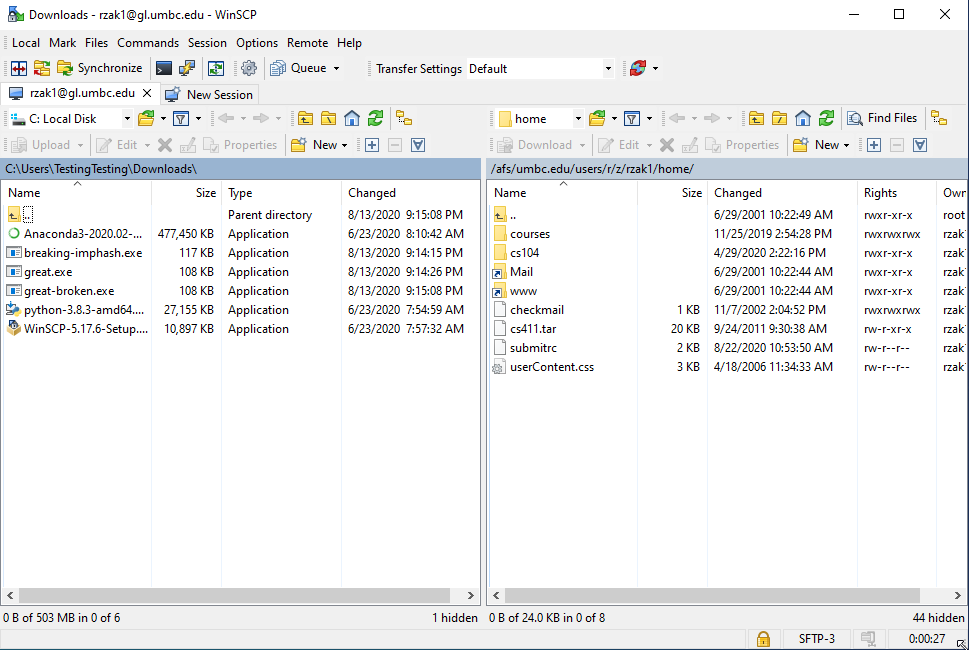
\includegraphics[scale=0.6]{Images/winscp_connected.png}
\caption{WinSCP showing local and remote files.}
\label{fig:winscpconnected}
\end{figure}

\FloatBarrier
\subsection{Mac Users}
\subsubsection{Terminal.app}
\paragraph{}The Mac operating system comes from a strong UNIX legacy. As such, the required components to interact with Linux servers at UMBC are already installed and ready to go! You'll use the Terminal application to connect to UMBC's servers. You can easily find the Terminal by navigating to Applications $\,\to\,$ Utilities, as shown in \autoref{fig:macfinderterminal} or by using Spotlight by pressing 
\includegraphics[height=.75em]{Images/command.eps} Space and begin typing Terminal, as shown in \autoref{fig:macspotlightterminal}.

\paragraph{}Once Terminal is open, type: \texttt{ssh userName@gl.umbc.edu} and press enter. Enter your password when prompted, and note that the password is shown. An example is shown in \autoref{fig:macterminalconnected}. For convenience, you can keep the Terminal icon in the Dock for future use. Right-Click on the Terminal icon, select Options $\,\to\,$ Keep in Dock, as shown in \autoref{fig:macterminaldock}.

\begin{figure}
\centering
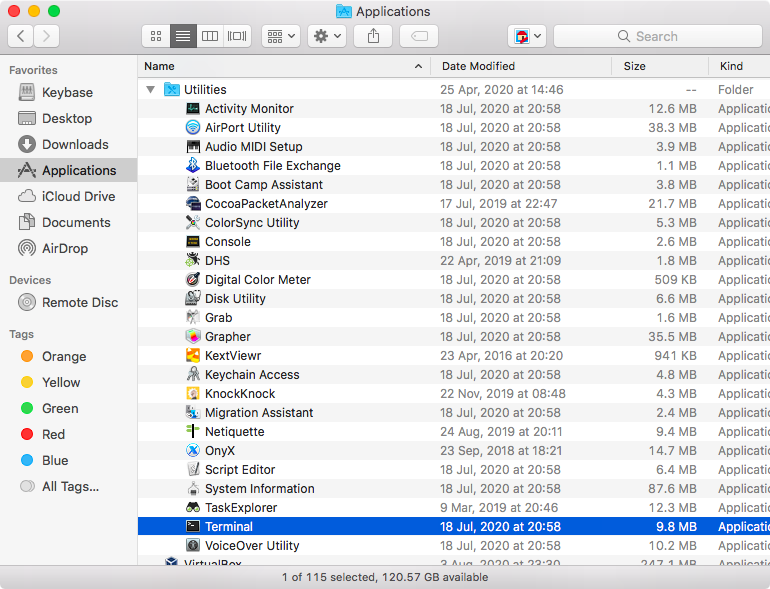
\includegraphics[scale=0.6]{Images/finder_terminal.png}
\caption{Finding Terminal with Finder.}
\label{fig:macfinderterminal}
\end{figure}

\begin{figure}
\centering
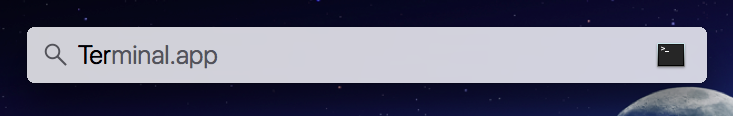
\includegraphics[scale=0.6]{Images/spotlight_terminal.png}
\caption{Searching for Terminal with Spotlight.}
\label{fig:macspotlightterminal}
\end{figure}

\begin{figure}
\centering
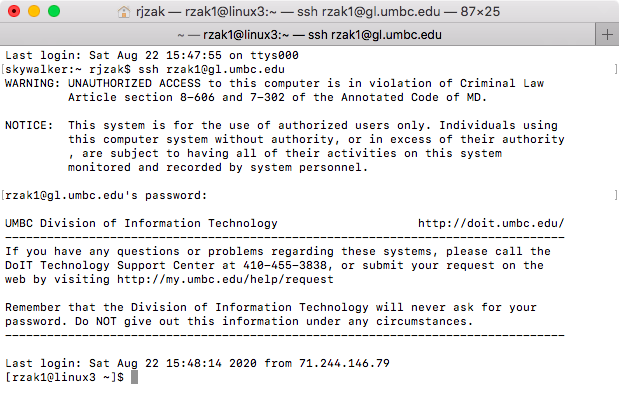
\includegraphics[scale=0.6]{Images/macos_terminal_ssh.png}
\caption{Terminal showing the SSH connection.}
\label{fig:macterminalconnected}
\end{figure}

\begin{figure}
\centering
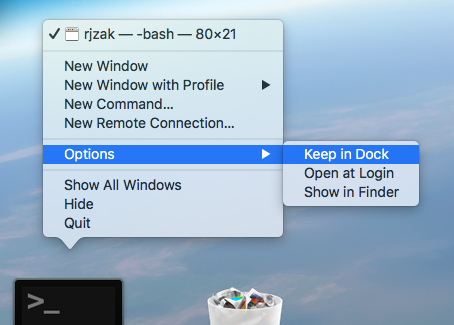
\includegraphics[scale=0.6]{Images/terminal_keep_in_dock.png}
\caption{Keeping the Terminal icon in the Dock for future use.}
\label{fig:macterminaldock}
\end{figure}

\FloatBarrier
\subsubsection{CyberDuck}
\paragraph{}CyberDuck is a graphical application for moving files between your Mac and other servers. It's available for download from \url{https://cyberduck.io/download/}.

\begin{enumerate}
    \item Download and install CyberDuck. You'll need to double-click the downloaded Zip file and drag-and-drop the CyberDuck application to the Applications directory.
    \item Run CyberDuck
    \item Click the icon to create a new connection. Make sure that the top pull-down menu says ``SFTP (SSH File Transfer Protocol)''. Enter ``gl.umbc.edu'' for the \texttt{Server} field, and your user name and password in the respective fields. Click ``Add to Keychain'' if you want Mac OS to store your password for future use. Click ``Connect''. An example is shown in \autoref{fig:maccyberduckconnect}.
    \item The first time you connect, you'll be prompted to accept the server's SSH key, as shown in \autoref{fig:maccyberduckconnectfirsttime}. Check the box that says ``Always'', and click ``Allow''.
    \item Now that you're connected, you'll see the files you have on the GL system, as shown in \autoref{fig:maccyberduckconnected}. You can drag-and-drop files to \& from the GL system.
\end{enumerate}

\begin{figure}
\centering
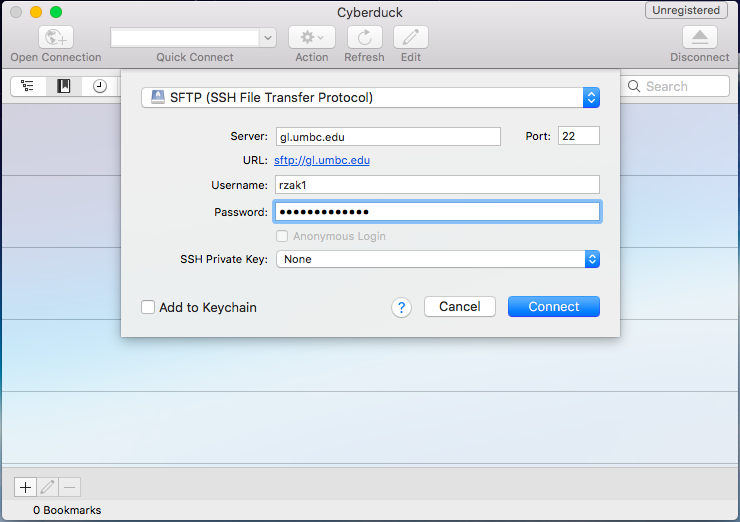
\includegraphics[scale=0.6]{Images/macos_cyberduck_connect.png}
\caption{Connecting to GL with CyberDuck.}
\label{fig:maccyberduckconnect}
\end{figure}

\begin{figure}
\centering
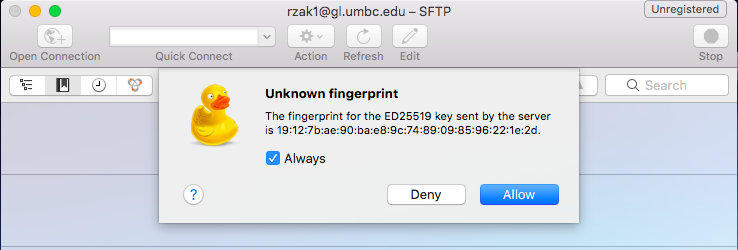
\includegraphics[scale=0.6]{Images/macos_cyberduck_firsttime.png}
\caption{CyberDuck asking about the server's SSH key.}
\label{fig:maccyberduckconnectfirsttime}
\end{figure}

\begin{figure}
\centering
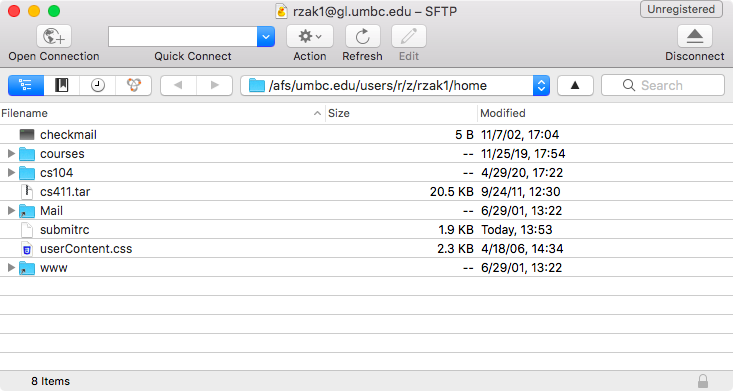
\includegraphics[scale=0.6]{Images/macos_cyberduck_connected.png}
\caption{CyberDuck asking about the server's SSH key.}
\label{fig:maccyberduckconnected}
\end{figure}

\FloatBarrier
\subsection{Extras}
\subsection{Shortcuts}
\paragraph{}Left as an exercise to the reader, Putty, WinSCP, and CyberDuck allow shortcuts. This allows you to easily reconnect to the UMBC GL servers without having to re-type the server name and your credentials.

\subsection{SSH Keys}
\paragraph{}Even after connecting for the first time, you may get a message about accepting SSH keys. This is expected for two reasons:

\begin{enumerate}
    \item The GL system consists of a few different Linux servers, and the GL system decided at connect time which one you'll be connecting to. For our purposes, it doesn't matter which you use, as they all will have your files, and all contain the programs we need.
    \item Sometimes, especially after an update on the server side, the SSH keys may change. It's not a cause for concern.
\end{enumerate}

\FloatBarrier
\section{Common Linux Commands}
\paragraph{Prompt}Once you're connected to the Linux server, you're presented with a command prompt. The prompt can look different depending on a few factors.

\begin{itemize}
\item {\color{red}31/Aug 21:55:45} {\color{green}rjzak@oryx-pro}:{\color{blue}{\raise.17ex\hbox{$\scriptstyle\sim$}}}\$
\item \texttt{[rzak1@linux3 {\raise.17ex\hbox{$\scriptstyle\sim$}}] \$}
\item \texttt{sh-5.0 \$}
\item \texttt{\$}
\end{itemize}

\paragraph{}All of these are examples of the Linux command prompt. What's interesting is that this is something which can be customized to display a variety of things, or can be extremely minimalistic and show you nothing. The first two indicate that the user name is \texttt{rjzak} and \texttt{rzak1} respectively. The first one has been customized to show the date, in addition to the user name and current location. Do you notice the {\raise.17ex\hbox{$\scriptstyle\sim$}} character? That is the shortcut for the user's home directory on the server. The symbol \texttt{\$} shows the end of the command prompt, and commands you type will appear here.

\subsection{Navigation}
\begin{itemize}
    \item \texttt{cd {\raise.17ex\hbox{$\scriptstyle\sim$}}}: Chane directory back to your home directory.
    \item \texttt{cd dirName}: Change to the directory called ``dirName''.
    \begin{itemize}
        \item \texttt{[rzak1@linux1 {\raise.17ex\hbox{$\scriptstyle\sim$}}]\$ cd /usr/sbin}
        \item \texttt{[rzak1@linux1 sbin]\$}
    \end{itemize}
    \item \texttt{pwd}: Print working directory. Where are you?
    \begin{itemize}
        \item \texttt{[rzak1@linux1 sbin]\$ pwd}
        \item \texttt{/usr/sbin}
    \end{itemize}
    \item \texttt{mkdir dirName}: Creates a directory called ``dirName''.
    \item \texttt{rm filename.ext}: Deletes a file called ``filename.ext''.
    \item \texttt{rm -r dirName}: Deletes a directory called ``dirName''. Note the \texttt{-r} option, it deletes the directory and everything contained within.
    \item \texttt{ls}: Get a listing of everything in a directory.
    \item \texttt{ls -lah}: Get a listing of everything in a directory, showing file sizes and creation time. Example:
    \begin{verbatim}
$ ls -lah Resume.pdf 
-rw-r--r-- 1 rjzak rjzak 97K Dec  5  2012 Resume.pdf\end{verbatim}
    \begin{itemize}
        \item My resume is 97 kilobytes in size, and hasn't been updated since 2012!
    \end{itemize}
\end{itemize}

\FloatBarrier
\subsubsection{File Systems}
\paragraph{}To better understand navigating, let's discuss what a file system is. A file system is the organization of files \& directories on a physical disk, and how this information is made available to the user of the machine, and to other applications which may be running. This layout forms a tree of files \& directories inside a directory, and it's not clear from looking at it if there is one of many hard drives used. This is in contrast to Windows, which uses drive labels, such as \texttt{A:} for a 3.5'' floppy drive (recognized today as ``the save icon''), \texttt{B:} for the ancient 5.24'' floppy drive, \texttt{C:} for the first hard drive, \texttt{D:} for the second hard drive, or optical disc, and further drives if attached to the computer.

\paragraph{}Example:
\begin{itemize}
    \item \texttt{sh-5.0 \$ mount}
    \begin{itemize}
        \item \texttt{/dev/sdb3 on / type ext4 (rw,relatime,errors=remount-ro,stripe=64,data=ordered)
}
        \item \texttt{/dev/sdb2 on /boot type ext4 (rw,relatime,stripe=64,data=ordered)}
        \item \texttt{/dev/sda1 on /datafs type ext4 (rw,nodev,noexec,relatime,stripe=256,data=ordered)}
    \end{itemize}
    \item \texttt{sh-5.0 \$ df -h}
    \begin{verbatim}
    Filesystem      Size  Used Avail Use% Mounted on
    /dev/sdb3       917G  454G  417G  53% /
    /dev/sdb2       923M  163M  698M  19% /boot
    /dev/sda1        39T   28T  9.3T  75% /datafs
    \end{verbatim}
    \item What does it mean?
    \begin{itemize}
        \item The root directory is the hard drive from \texttt{/dev/sdb3}. Physical devices are files in Unix.
        \item The file system used here is called \texttt{ext4}, which is how the actual data on the physical hard drive is organized. There are many different types of file systems, and with Linux and Unix, they're very similar between different operating systems and their variations. Wikipedia has an article here: \url{https://en.wikipedia.org/wiki/File_system}.
        \item The \texttt{df -h} shows the amount of free and used disk space, and \texttt{-h} means to show the results in a human-readable display, using MB, GB, TB instead of very large numbers which are harder to interpret. 923 M (for megabytes, MB, is equal to 967,835,648 bytes, which is easier to read and comprehend at a glance?
    \end{itemize}
\end{itemize}

\FloatBarrier
\begin{figure}
% Copyright 2002-2023 The University of Maryland Baltimore County (UMBC)
% 1000 Hilltop Circle, Baltimore, Maryland, 21250, USA
% https://www.csee.umbc.edu/

% Graphic for TeX using PGF
% Title: /home/rjzak/Dropbox/School/Teaching/CMSC104/UnixFS.dia
% Creator: Dia v0.97+git
% CreationDate: Mon Aug 31 22:40:12 2020
% For: rjzak
% \usepackage{tikz}
% The following commands are not supported in PSTricks at present
% We define them conditionally, so when they are implemented,
% this pgf file will use them.

\ifx\du\undefined
  \newlength{\du}
\fi
\setlength{\du}{15\unitlength}
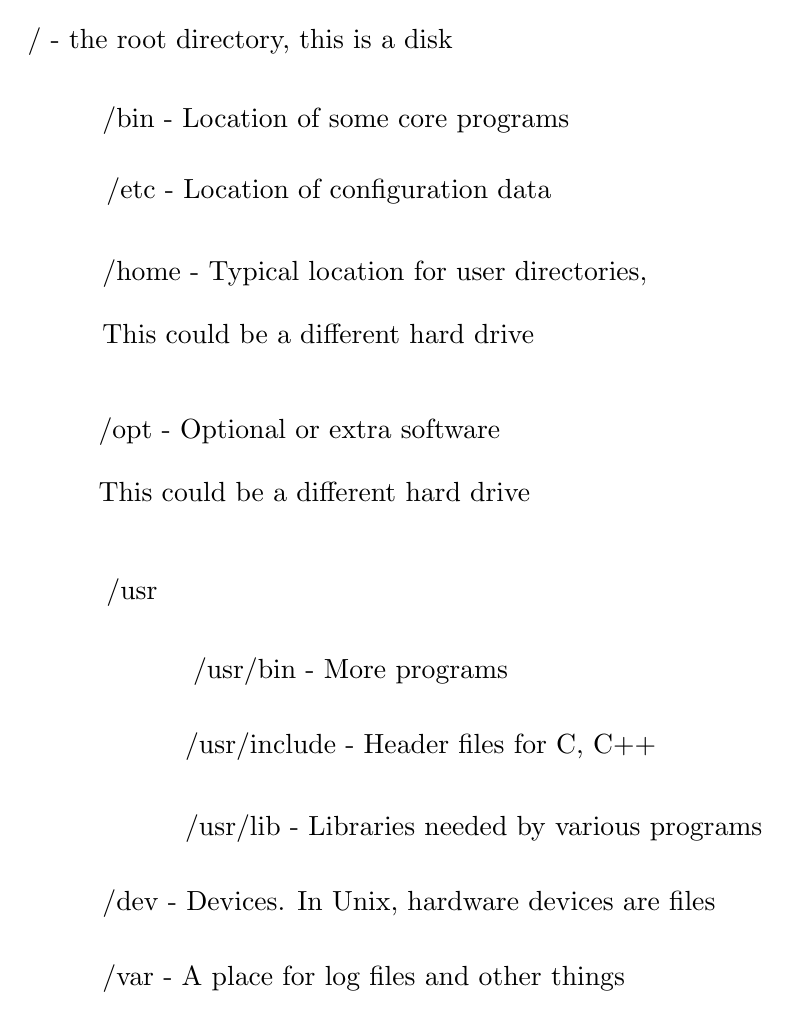
\begin{tikzpicture}[even odd rule]
\pgftransformxscale{1.000000}
\pgftransformyscale{-1.000000}
\definecolor{dialinecolor}{rgb}{0.000000, 0.000000, 0.000000}
\pgfsetstrokecolor{dialinecolor}
\pgfsetstrokeopacity{1.000000}
\definecolor{diafillcolor}{rgb}{1.000000, 1.000000, 1.000000}
\pgfsetfillcolor{diafillcolor}
\pgfsetfillopacity{1.000000}
% setfont left to latex
\definecolor{dialinecolor}{rgb}{0.000000, 0.000000, 0.000000}
\pgfsetstrokecolor{dialinecolor}
\pgfsetstrokeopacity{1.000000}
\definecolor{diafillcolor}{rgb}{0.000000, 0.000000, 0.000000}
\pgfsetfillcolor{diafillcolor}
\pgfsetfillopacity{1.000000}
\node[anchor=base west,inner sep=0pt,outer sep=0pt,color=dialinecolor] at (1.300000\du,1.800000\du){/ - the root directory, this is a disk};
% setfont left to latex
\definecolor{dialinecolor}{rgb}{0.000000, 0.000000, 0.000000}
\pgfsetstrokecolor{dialinecolor}
\pgfsetstrokeopacity{1.000000}
\definecolor{diafillcolor}{rgb}{0.000000, 0.000000, 0.000000}
\pgfsetfillcolor{diafillcolor}
\pgfsetfillopacity{1.000000}
\node[anchor=base west,inner sep=0pt,outer sep=0pt,color=dialinecolor] at (2.250000\du,2.800000\du){/bin - Location of some core programs};
% setfont left to latex
\definecolor{dialinecolor}{rgb}{0.000000, 0.000000, 0.000000}
\pgfsetstrokecolor{dialinecolor}
\pgfsetstrokeopacity{1.000000}
\definecolor{diafillcolor}{rgb}{0.000000, 0.000000, 0.000000}
\pgfsetfillcolor{diafillcolor}
\pgfsetfillopacity{1.000000}
\node[anchor=base west,inner sep=0pt,outer sep=0pt,color=dialinecolor] at (2.300000\du,3.700000\du){/etc - Location of configuration data};
% setfont left to latex
\definecolor{dialinecolor}{rgb}{0.000000, 0.000000, 0.000000}
\pgfsetstrokecolor{dialinecolor}
\pgfsetstrokeopacity{1.000000}
\definecolor{diafillcolor}{rgb}{0.000000, 0.000000, 0.000000}
\pgfsetfillcolor{diafillcolor}
\pgfsetfillopacity{1.000000}
\node[anchor=base west,inner sep=0pt,outer sep=0pt,color=dialinecolor] at (2.250000\du,4.750000\du){/home - Typical location for user directories,};
% setfont left to latex
\definecolor{dialinecolor}{rgb}{0.000000, 0.000000, 0.000000}
\pgfsetstrokecolor{dialinecolor}
\pgfsetstrokeopacity{1.000000}
\definecolor{diafillcolor}{rgb}{0.000000, 0.000000, 0.000000}
\pgfsetfillcolor{diafillcolor}
\pgfsetfillopacity{1.000000}
\node[anchor=base west,inner sep=0pt,outer sep=0pt,color=dialinecolor] at (2.250000\du,5.550000\du){             This could be a different hard drive};
% setfont left to latex
\definecolor{dialinecolor}{rgb}{0.000000, 0.000000, 0.000000}
\pgfsetstrokecolor{dialinecolor}
\pgfsetstrokeopacity{1.000000}
\definecolor{diafillcolor}{rgb}{0.000000, 0.000000, 0.000000}
\pgfsetfillcolor{diafillcolor}
\pgfsetfillopacity{1.000000}
\node[anchor=base west,inner sep=0pt,outer sep=0pt,color=dialinecolor] at (2.200000\du,6.750000\du){/opt - Optional or extra software};
% setfont left to latex
\definecolor{dialinecolor}{rgb}{0.000000, 0.000000, 0.000000}
\pgfsetstrokecolor{dialinecolor}
\pgfsetstrokeopacity{1.000000}
\definecolor{diafillcolor}{rgb}{0.000000, 0.000000, 0.000000}
\pgfsetfillcolor{diafillcolor}
\pgfsetfillopacity{1.000000}
\node[anchor=base west,inner sep=0pt,outer sep=0pt,color=dialinecolor] at (2.200000\du,7.550000\du){         This could be a different hard drive};
% setfont left to latex
\definecolor{dialinecolor}{rgb}{0.000000, 0.000000, 0.000000}
\pgfsetstrokecolor{dialinecolor}
\pgfsetstrokeopacity{1.000000}
\definecolor{diafillcolor}{rgb}{0.000000, 0.000000, 0.000000}
\pgfsetfillcolor{diafillcolor}
\pgfsetfillopacity{1.000000}
\node[anchor=base west,inner sep=0pt,outer sep=0pt,color=dialinecolor] at (2.300000\du,8.800000\du){/usr};
% setfont left to latex
\definecolor{dialinecolor}{rgb}{0.000000, 0.000000, 0.000000}
\pgfsetstrokecolor{dialinecolor}
\pgfsetstrokeopacity{1.000000}
\definecolor{diafillcolor}{rgb}{0.000000, 0.000000, 0.000000}
\pgfsetfillcolor{diafillcolor}
\pgfsetfillopacity{1.000000}
\node[anchor=base west,inner sep=0pt,outer sep=0pt,color=dialinecolor] at (3.400000\du,9.800000\du){/usr/bin - More programs};
% setfont left to latex
\definecolor{dialinecolor}{rgb}{0.000000, 0.000000, 0.000000}
\pgfsetstrokecolor{dialinecolor}
\pgfsetstrokeopacity{1.000000}
\definecolor{diafillcolor}{rgb}{0.000000, 0.000000, 0.000000}
\pgfsetfillcolor{diafillcolor}
\pgfsetfillopacity{1.000000}
\node[anchor=base west,inner sep=0pt,outer sep=0pt,color=dialinecolor] at (3.300000\du,10.750000\du){/usr/include - Header files for C, C++};
% setfont left to latex
\definecolor{dialinecolor}{rgb}{0.000000, 0.000000, 0.000000}
\pgfsetstrokecolor{dialinecolor}
\pgfsetstrokeopacity{1.000000}
\definecolor{diafillcolor}{rgb}{0.000000, 0.000000, 0.000000}
\pgfsetfillcolor{diafillcolor}
\pgfsetfillopacity{1.000000}
\node[anchor=base west,inner sep=0pt,outer sep=0pt,color=dialinecolor] at (3.300000\du,11.800000\du){/usr/lib - Libraries needed by various programs};
% setfont left to latex
\definecolor{dialinecolor}{rgb}{0.000000, 0.000000, 0.000000}
\pgfsetstrokecolor{dialinecolor}
\pgfsetstrokeopacity{1.000000}
\definecolor{diafillcolor}{rgb}{0.000000, 0.000000, 0.000000}
\pgfsetfillcolor{diafillcolor}
\pgfsetfillopacity{1.000000}
\node[anchor=base west,inner sep=0pt,outer sep=0pt,color=dialinecolor] at (2.250000\du,12.750000\du){/dev - Devices. In Unix, hardware devices are files};
% setfont left to latex
\definecolor{dialinecolor}{rgb}{0.000000, 0.000000, 0.000000}
\pgfsetstrokecolor{dialinecolor}
\pgfsetstrokeopacity{1.000000}
\definecolor{diafillcolor}{rgb}{0.000000, 0.000000, 0.000000}
\pgfsetfillcolor{diafillcolor}
\pgfsetfillopacity{1.000000}
\node[anchor=base west,inner sep=0pt,outer sep=0pt,color=dialinecolor] at (2.250000\du,13.700000\du){/var - A place for log files and other things};
\end{tikzpicture}

\caption{A basic Unix filesystem layout}
\label{fig:unixfs}
\end{figure}

\FloatBarrier
\subsection{Files}
\begin{itemize}
    \item \texttt{head}: Show the beginning of a file. Optionally see the first XX lines by typing \texttt{head -n XX file.txt}.
    \item \texttt{tail}: Show the end of a file. Optionally see the last XX lines by typing \texttt{tail -n XX file.txt}, or monitor the file by typing \texttt{tail -f file.txt}.
    \item \texttt{xxd}: Show the contents of a binary file. Works well when used with \texttt{head} or \texttt{tail}, such as \texttt{xxd someFile.bin | head -n 2} to see the first two lines of the binary file.
\end{itemize}

\FloatBarrier
\subsection{Submit}
\paragraph{}Many computer science courses use the \texttt{submit} system to receive assignments from students.
\begin{itemize}
    \item \texttt{submit cs104\_1234 proj1 file1.c file2.txt...}: Submit the files for, in this case ``proj1'' to the course listed. The course names and assignments will be provided by your instructor and is \textbf{DIFFERENT FOR EACH COURSE AND SECTION!}
    \item \texttt{submitls cs104\_1234 proj1}: List the files that you've submitted for your course and assignment. Note the important bold notice above.
\end{itemize}

\FloatBarrier
\subsection{Miscellaneous}
\begin{itemize}
    \item \texttt{uptime}: How long has the machine been running?
    \begin{itemize}
        \item \texttt{[rzak1@linux1 {\raise.17ex\hbox{$\scriptstyle\sim$}}]\$ uptime}
        \item \texttt{22:18:45 up 14 days, 37 min, 25 users,  load average: 0.24, 1.23, 1.13}
    \end{itemize}
    \item \texttt{file filename.ext}
    \begin{verbatim}
$ file myProgram resume
myProgram: ELF 64-bit LSB executable, x86-64, version 1 (SYSV), statically linked
resume: PDF document, version 1.4\end{verbatim}
    \item What does it mean?
    \begin{itemize}
        \item \texttt{ELF} is the Executable and Linkable Format, the file format used by most Unix systems, including Linux. Wikipedia link: \url{https://en.wikipedia.org/wiki/Executable\_and\_Linkable\_Format}.
        \item \texttt{x86-64} shows that the program is 64-bit and runs on Intel processors, the most common processor in consumer computers.
        \item The \texttt{file} command can determine the type of file even when the file extension is missing, showing that my resume is actually a PDF file.
    \end{itemize}
    \item \texttt{uname -a}: Show the version of the Kernel (the brains of the operating system)
    \begin{verbatim}
$ uname -a
Linux linux1.gl.umbc.edu 5.7.14-200.fc32.x86_64 #1 SMP Fri Aug 7 23:16:37 UTC 2020 x86_64
x86_64 x86_64 GNU/Linux\end{verbatim}
\end{itemize}

\FloatBarrier
\section{Trying Linux on your device}
\paragraph{}Linux, like many things, is best learned by using it often. If you are interested in learning how to use Linux, you might want to try running Linux on your own machine instead of connecting to UMBC. This will also show you the graphical interface, which you're missing out on when using SSH. Linux is free and open source software (FOSS), so trying it on your own machine doesn't cost anything.

\paragraph{}Being proficient with Linux, or at least having some experience with Linux, is a worthwhile and sought-after skill. This is something worth learning and putting on your resume. While Windows may be the dominant operating system for desktops at home and in the office, Linux is popular in a few domains which include: software development, high performance computing, embedded systems, automotive, life sciences, oil \& gas exploration, weather modeling, computer networking, forensics, cybersecurity, and more.

\begin{enumerate}
    \item Download an install a \textit{hypervisor}, which is the software which runs a virtual machine. VirtualBox is recommended since it's free, easy to use, and runs on most operating systems. Download it from \url{http://virtualbox.org/} and install.
    \item Pick a \textit{distribution} to test. Ubuntu or Linux Mint are recommended, since they're easy to install and get running.
    \begin{itemize}
        \item Ubuntu: \url{http://ubuntu.com/}
        \item Linux Mint: \url{https://linuxmint.com/}
        \item When you decide on which distribution, look for a link that says Download, and find a link for an ISO file (ends with .iso). 
    \end{itemize}
    \item Create a new Virtual Machine
    \begin{enumerate}
        \item Click the new VM icon
        \item Pick the operating system
        \item Show VirtualBox where the ISO file is you downloaded.
    \end{enumerate}
\end{enumerate}

\subsection{Virtual Machine}
\paragraph{}The easiest option is to install Linux in a virtual machine (VM). You can install Linux into a new VM, or you can find pre-made VMs available for your use. It's best to install Linux into a VM yourself so you have a deeper understanding and appreciation for Linux and how it works, but it's your choice.

\FloatBarrier
\subsection{Linux on Windows 10}
\paragraph{}Recent versions of Windows 10 allow for the installation of Microsoft's Windows Subsystem for Linux (WSL). It's esentially a virtual machine, but with a custom Linux kernel which communicates with the Windows kernel. Installing WSL requires a Microsoft account and signing in to the Microsoft app store.

\begin{enumerate}
    \item Open the Microsoft Windows app store and search for Linux. \autoref{fig:wslsearchlinux} shows an example of what this looks like.
    \item Select Ubuntu.
    \item Click install. It download and installs quickly. Soon you'll see a notification just like \autoref{fig:wslinstalled}.
    \item In the notification in the prior step, or from the Ubuntu app in the start menu, launch Ubuntu. For the first run, you'll see another installation screen, as shown in \autoref{fig:wslinstallparttwo}.
    \item After secondary installation completes, pick a user name and password, and you've got Linux on Windows! See \autoref{fig:wslinstallcomplete}.
    \item Customize your WSL:
    \begin{itemize}
        \item Run \texttt{sudo apt-get update} and \texttt{sudo apt-get dist-upgrade} to make sure it's fully up-to-date.
        \item To install compilers and software development tools, run \texttt{sudo apt-get install build-essential}.
        \item You should be able to run \texttt{nano} to create text files, which include source code and Makefiles.
        \item Navigate to \texttt{/mnt/c/} to access drive \texttt{C:} from Linux. This shows how you can access your regular home directory, or other locations on \texttt{C:} from WSL. It makes it easier to move data around. See \autoref{fig:wsldrivec}.
        \item You can directly SSH to UMBC from WSL, no Putty needed!
    \end{itemize}
\end{enumerate}

\begin{figure}
    \centering
    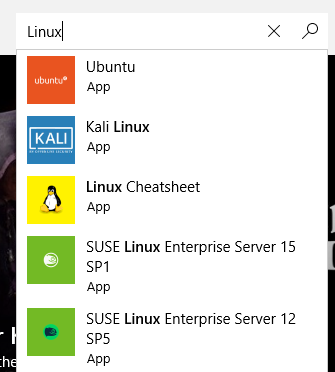
\includegraphics[scale=0.6]{Images/WSL/a.png}
    \caption{Search for Linux}
    \label{fig:wslsearchlinux}
\end{figure}

\begin{figure}
    \centering
    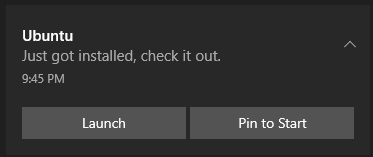
\includegraphics[scale=0.6]{Images/WSL/b.png}
    \caption{Ubuntu installed successfully}
    \label{fig:wslinstalled}
\end{figure}

\begin{figure}
    \centering
    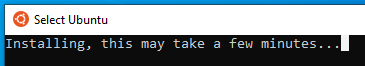
\includegraphics[scale=0.8]{Images/WSL/c.png}
    \caption{Ubuntu installation part two}
    \label{fig:wslinstallparttwo}
\end{figure}

\begin{figure}
    \centering
    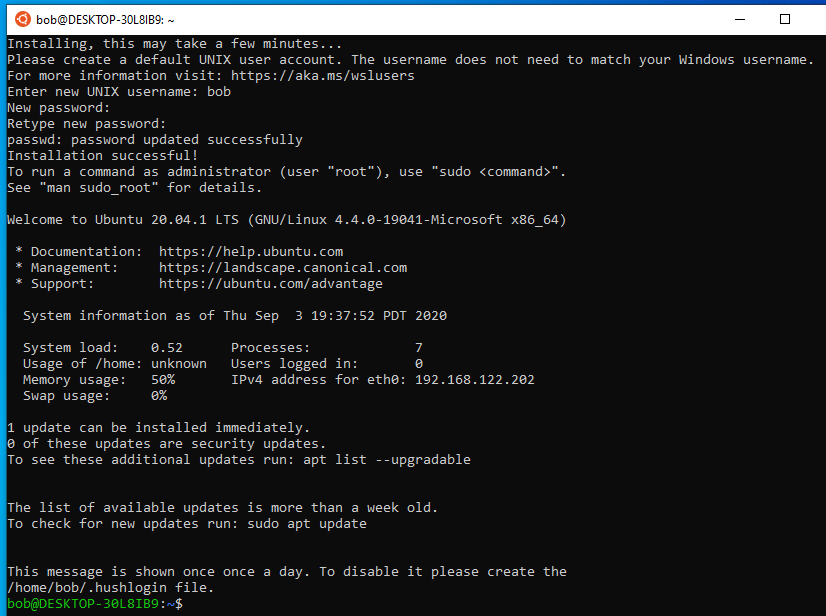
\includegraphics[scale=0.64]{Images/WSL/d.png}
    \caption{Ubuntu installed}
    \label{fig:wslinstallcomplete}
\end{figure}

\begin{figure}
    \centering
    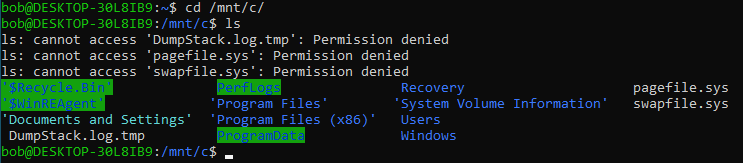
\includegraphics[scale=0.64]{Images/WSL/e.png}
    \caption{Access drive C: from WSL}
    \label{fig:wsldrivec}
\end{figure}

\FloatBarrier

\section{UMBC Linux Users Group (LUG)}
\paragraph{}There is a Linux Users Group at UMBC, connect with them via the links below. It's a great way to learn more about Linux from fellow students.
\begin{itemize}
    \item My UMBC: \url{https://my3.my.umbc.edu/groups/lug}
    \item Discord: \url{https://discord.gg/3XrJe465Wz}
\end{itemize}

\end{document}